\documentclass[tikz, border=3mm]{standalone}
\usepackage{tikz}
\usetikzlibrary{arrows.meta}

\begin{document}
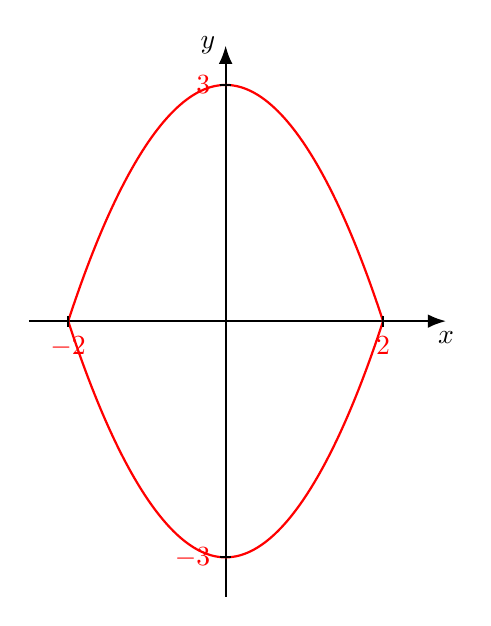
\begin{tikzpicture}[
    >=Latex, % Set default arrow tip style
    labelstyle/.style={red}, % Style for labels
    tick/.style={thick} % Style for tick marks
]

    % Axes
    \draw[->, thick] (-2.5, 0) -- (2.8, 0) node[below] {$x$};
    \draw[->, thick] (0, -3.5) -- (0, 3.5) node[left] {$y$};

    % Define key points (intersections with axes)
    \coordinate (L) at (-2, 0); % Left point
    \coordinate (R) at (2, 0);  % Right point
    \coordinate (T) at (0, 3);  % Top point (vertex of top parabola)
    \coordinate (B) at (0, -3); % Bottom point (vertex of bottom parabola)

    % Draw the red shape using PARABOLAS with specified bend (vertex)
    % Top parabola: Starts at L, ends at R, vertex at T
    \draw[red, thick] (L) parabola [bend = (T)] (R);
    % Bottom parabola: Starts at L, ends at R, vertex at B
    \draw[red, thick] (L) parabola [bend = (B)] (R);

    % --- Add Ticks and Labels at ALL intersection points ---
    % Ticks on x-axis
    \draw[tick] (L) ++(0,-2pt) -- ++(0,4pt); % Vertical tick at x=-2
    \draw[tick] (R) ++(0,-2pt) -- ++(0,4pt); % Vertical tick at x=2

    % Ticks on y-axis
    \draw[tick] (T) ++(-2pt,0) -- ++(4pt,0); % Horizontal tick at y=3
    \draw[tick] (B) ++(-2pt,0) -- ++(4pt,0); % Horizontal tick at y=-3

    % Labels for ticks
    \node[labelstyle, below=2pt] at (L) {$-2$};
    \node[labelstyle, below=2pt] at (R) {$2$};
    \node[labelstyle, left=2pt] at (T) {$3$};
    \node[labelstyle, left=2pt] at (B) {$-3$};
    % --- End Ticks and Labels ---

\end{tikzpicture}
\end{document}